\documentclass[11pt,addpoints]{exam}

\usepackage[margin=1in]{geometry}
\usepackage{amsmath,amssymb}
\usepackage{tikz}
\usepackage{enumitem}
\usepackage{multicol}

% Header and footer
\pagestyle{headandfoot}
\firstpageheader{Algebra II \& Trigonometry}{Quiz 4}{Room 214 -- Ms.\ Thornton}
\runningheader{Algebra II \& Trigonometry}{Quiz 4}{Page \thepage\ of \numpages}
\firstpagefooter{}{}{}
\runningfooter{}{}{}
\firstpageheadrule
\runningheadrule

\pointpoints{point}{points}
\qformat{\textbf{Question \thequestion} \quad (\totalpoints\ \points)\hfill}

\begin{document}

\begin{center}
  {\Large\bfseries Quiz 4: Quadratic Functions and Right-Triangle Trigonometry}\\[8pt]
  \makebox[0.55\textwidth]{Name:\enspace\hrulefill}
  \qquad
  \makebox[0.25\textwidth]{Date:\enspace\hrulefill}
\end{center}

\vspace{4pt}
\noindent\textbf{Instructions.} You have 40 minutes. Show all work for full credit; a correct answer with no work earns at most half the points. Calculators are allowed. Round decimal answers to two decimal places unless told otherwise. Angles are in degrees.

\begin{center}
  \gradetable[h][questions]
\end{center}

\begin{questions}

%-------------------------------------------------------------------------
\question[2]
What is the vertex of the parabola $y = 2(x - 3)^2 + 5$?
\begin{oneparchoices}
  \choice $(-3, 5)$
  \choice $(3, -5)$
  \choice $(3, 5)$
  \choice $(2, 5)$
\end{oneparchoices}

%-------------------------------------------------------------------------
\question[3]
Solve by factoring: $x^2 - 5x + 6 = 0$.
\vspace{2.5cm}

%-------------------------------------------------------------------------
\question[4]
Use the quadratic formula to solve $2x^2 + 3x - 4 = 0$. Give exact answers in simplest radical form, then approximate each to two decimal places.
\vspace{3.5cm}

%-------------------------------------------------------------------------
\question[3]
Without solving, use the discriminant to determine how many real solutions $3x^2 - 2x + 5 = 0$ has. Explain your reasoning in one sentence.
\vspace{2.5cm}

%-------------------------------------------------------------------------
\question[4]
Rewrite $f(x) = x^2 + 6x + 2$ in vertex form by completing the square. Then state the vertex and the equation of the axis of symmetry.
\vspace{3cm}

%-------------------------------------------------------------------------
\question
A ball is thrown upward from the top of a 5-foot platform. Its height, in feet, after $t$ seconds is
\[
  h(t) = -16t^2 + 64t + 5.
\]
\begin{parts}
  \part[2] How high is the ball after 1 second?
  \vspace{1.8cm}
  \part[3] When does the ball reach its maximum height, and what is that height?
  \vspace{2.5cm}
  \part[3] After how many seconds does the ball hit the ground? Round to the nearest hundredth.
  \vspace{3cm}
\end{parts}

\newpage
%-------------------------------------------------------------------------
\question
In right triangle $ABC$ below, $\angle C = 90^\circ$, $\angle A = 35^\circ$, and the hypotenuse $AB = 12$.

\begin{center}
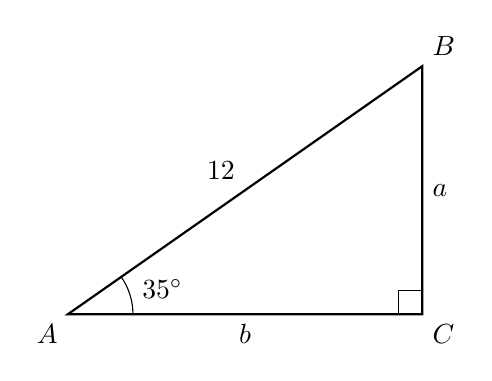
\begin{tikzpicture}[scale=0.75, thick]
  \coordinate (A) at (0,0);
  \coordinate (C) at (6,0);
  \coordinate (B) at (6,4.2);
  \draw (A) -- (C) -- (B) -- cycle;
  % right-angle marker at C
  \draw[thin] (C) ++(-0.4,0) -- ++(0,0.4) -- ++(0.4,0);
  % angle arc at A
  \draw[thin] (1.1,0) arc[start angle=0, end angle=35, radius=1.1];
  \node at (1.6,0.42) {$35^\circ$};
  \node[below left]  at (A) {$A$};
  \node[below right] at (C) {$C$};
  \node[above right] at (B) {$B$};
  \node[above left]  at (3,2.1) {$12$};
  \node[right]       at (6,2.1) {$a$};
  \node[below]       at (3,0)   {$b$};
\end{tikzpicture}
\end{center}

\begin{parts}
  \part[3] Find the length of side $a$ (opposite $\angle A$).
  \vspace{2cm}
  \part[3] Find the length of side $b$ (adjacent to $\angle A$).
  \vspace{2cm}
  \part[1] What is the measure of $\angle B$?
  \vspace{1.2cm}
\end{parts}

%-------------------------------------------------------------------------
\question[4]
A 15-foot ladder leans against a vertical wall. The top of the ladder touches the wall 13 feet above the ground. What angle does the ladder make with the ground? Draw and label a diagram.
\vspace{4cm}

%-------------------------------------------------------------------------
\question[3]
Give the exact value of each expression (no decimals).
\begin{multicols}{3}
\begin{enumerate}[label=(\alph*)]
  \item $\sin 30^\circ$
  \item $\cos 45^\circ$
  \item $\tan 60^\circ$
\end{enumerate}
\end{multicols}
\vspace{1.5cm}

%-------------------------------------------------------------------------
\bonusquestion[2]
For what value(s) of $k$ does $x^2 + kx + 9 = 0$ have exactly one real solution?
\vspace{2.5cm}

\end{questions}

\begin{center}
  \textit{End of quiz. Check your work!}
\end{center}

%=========================================================================
\newpage
\begin{center}
  {\Large\bfseries Answer Key --- Quiz 4}\\[4pt]
  \textit{For teacher use only. Total: \numpoints\ points plus \numbonuspoints\ bonus.}
\end{center}

\begin{enumerate}[label=\textbf{\arabic*.}, leftmargin=*, itemsep=8pt]

  \item \textbf{(C)} $(3, 5)$. In vertex form $y = a(x-h)^2 + k$ the vertex is $(h, k)$.

  \item $(x - 2)(x - 3) = 0$, so $x = 2$ or $x = 3$.

  \item With $a = 2$, $b = 3$, $c = -4$:
  \[
    x = \frac{-3 \pm \sqrt{3^2 - 4(2)(-4)}}{2(2)} = \frac{-3 \pm \sqrt{41}}{4},
  \]
  so $x \approx 0.85$ or $x \approx -2.35$.

  \item $\Delta = b^2 - 4ac = (-2)^2 - 4(3)(5) = 4 - 60 = -56 < 0$, so there are \textbf{no real solutions}.

  \item $f(x) = (x^2 + 6x + 9) - 9 + 2 = (x + 3)^2 - 7$. Vertex $(-3, -7)$; axis of symmetry $x = -3$.

  \item
  \begin{enumerate}[label=(\alph*)]
    \item $h(1) = -16 + 64 + 5 = 53$ feet.
    \item $t = -\dfrac{b}{2a} = -\dfrac{64}{2(-16)} = 2$ seconds; $h(2) = -64 + 128 + 5 = 69$ feet.
    \item Solve $-16t^2 + 64t + 5 = 0$:
    \[
      t = \frac{-64 \pm \sqrt{64^2 - 4(-16)(5)}}{2(-16)} = \frac{-64 \pm \sqrt{4416}}{-32}.
    \]
    $\sqrt{4416} \approx 66.45$, giving $t \approx -0.08$ (reject, negative time) or $t \approx 4.08$ seconds.
  \end{enumerate}

  \item
  \begin{enumerate}[label=(\alph*)]
    \item $a = 12 \sin 35^\circ \approx 12(0.5736) \approx 6.88$.
    \item $b = 12 \cos 35^\circ \approx 12(0.8192) \approx 9.83$.
    \item $\angle B = 90^\circ - 35^\circ = 55^\circ$.
  \end{enumerate}
  \emph{Check:} $6.88^2 + 9.83^2 \approx 47.3 + 96.6 = 143.9 \approx 144 = 12^2$.

  \item The ladder is the hypotenuse and the height is opposite the angle $\theta$ at the ground:
  \[
    \sin\theta = \frac{13}{15} \quad\Longrightarrow\quad \theta = \sin^{-1}\!\left(\frac{13}{15}\right) \approx 60.07^\circ.
  \]
  Give full credit for $60.1^\circ$. Deduct 1 point if the diagram is missing or unlabeled.

  \item (a) $\dfrac{1}{2}$ \qquad (b) $\dfrac{\sqrt{2}}{2}$ \qquad (c) $\sqrt{3}$

  \item[\textbf{Bonus.}] Exactly one real solution requires $\Delta = k^2 - 4(1)(9) = 0$, so $k^2 = 36$ and $k = \pm 6$. (Both values needed for full bonus credit.)

\end{enumerate}

\vspace{6pt}
\noindent\textbf{Common errors to watch for:} sign errors in the vertex for question 1 (choice A); forgetting the $-9$ when completing the square; using $\cos$ instead of $\sin$ in question 8; calculators left in radian mode (gives $\sin 35 \approx -0.43$).

\end{document}
